\documentclass[10pt,twocolumn,letterpaper]{article}

\usepackage{cvpr}
\usepackage{times}
\usepackage{epsfig}
\usepackage{amsmath}
\usepackage{amssymb}

\usepackage{booktabs} % for much better looking tables
\usepackage{array} % for better arrays (eg matrices) in maths
\usepackage{paralist} % very flexible & customisable lists (eg. enumerate/itemize, etc.)
\usepackage{verbatim} % adds environment for commenting out blocks of text & for better verbatim
\usepackage{subfigure} % make it possible to include more than one captioned figure/table in a single float
\usepackage{graphicx}
\usepackage{epstopdf}
% Include other packages here, before hyperref.

% If you comment hyperref and then uncomment it, you should delete
% egpaper.aux before re-running latex.  (Or just hit 'q' on the first latex
% run, let it finish, and you should be clear).
%\usepackage[pagebackref=true,breaklinks=true,letterpaper=true,colorlinks,bookmarks=false]{hyperref}

\cvprfinalcopy % *** Uncomment this line for the final submission

\def\cvprPaperID{****} % *** Enter the CVPR Paper ID here
\def\httilde{\mbox{\tt\raisebox{-.5ex}{\symbol{126}}}}

% Pages are numbered in submission mode, and unnumbered in camera-ready
\ifcvprfinal\pagestyle{empty}\fi
\begin{document}

%%%%%%%%% TITLE
\title{
Project in CSE 250B\\
Assignment 1: Recognition of Handwritten Digits}

\author{Andreas Landstad, Spencer Bliven, Jonas Hoelzler\\
Computer Science Department\\
University of California, San Diego\\
{\tt\small landstad.andreas@gmail.com, sbliven@ucsd.edu, jonas@hoelzler.de}
}% For a paper whose authors are all at the same institution,
% omit the following lines up until the closing ``}''.
% Additional authors and addresses can be added with ``\and'',
% just like the second author.
% To save space, use either the email address or home page, not both
%\and
%Second Author\\
%Institution2\\
%First line of institution2 address\\
%{\tt\small secondauthor@i2.org}
\maketitle
\thispagestyle{empty}

%%%%%%%%% ABSTRACT
\begin{abstract}
For this project, different variants of nearest-neighbor classifiers for handwritten digit recognition are implemented and compared. The results are evaluated using the USPS dataset. It was found that the $k$-nearest-neighbor classification method (kNN) using Euclidean distance yields the lowest error rate of all implemented variants with 5.6\% error.
The weighted similarity function is slightly worse with 5.8\%.   
Both results are significantly worse than the best known classifiers, such as the classifier of Keysers et al. \cite{keysers}, which achieves an error rate of only 2.2\%.
\end{abstract}

%%%%%%%%% BODY TEXT
\section{Introduction}

\subsection{Nearest-Neighbor Classification}
Nearest-neighbor classification is a supervised learning method. As input, the algorithm takes a set of training examples and a set of query points. Training examples are pairs $\left( x,y \right) \in \mathbb{R}^m \times \mathcal{C}$, where $x$ is an $m$-dimensional point and $y$ is a label from some set of possible labels, $\mathcal{C}$. Query points are $m$-dimensional points $x \in \mathbb{R}^m$ with unknown labels. The goal is to predict labels for each query point. The nearest-neighbor classification method is one of the simplest of all supervised learning algorithms. The training phase is no more than storing every training example with its label. To make a prediction for a query point, one computes the distance from the query to every training example. In $k$-nearest-neighbor classification ($k$NN), the $k$ closest training examples to each query are considered, and a prediction for the query is made based on the labels for these points. The full procedure for predicting the label for the query is explained in detail in Section \ref{kNN}. Another major consideration in the implementation of $k$NN is selection of an appropriate distance function (Section \ref{distancefunctions}).
 

\subsection{The USPS dataset}
In this project the algorithms are applied to the multiclass learning problem of recognizing handwritten digits taken from the US Mail (Figure \ref{digits}).

The USPS dataset contains training and test data from normalized handwritten digits, automatically
scanned from envelopes by the U.S. Postal Service. The original scanned digits are binary and of different sizes and orientations; the images have been deslanted and size normalized, resulting in 16 x 16 grayscale images \cite{LeCun}. The image instances are represented by a vector with 256 features.
There are 7291 training observations and 2007 test observations. Digits are distributed roughly uniformly, with a bias towards zeros and ones (see Figure \ref{distribution}). 

\begin{figure}[htbp]
  \centering

    \begin{minipage}{8 cm}
      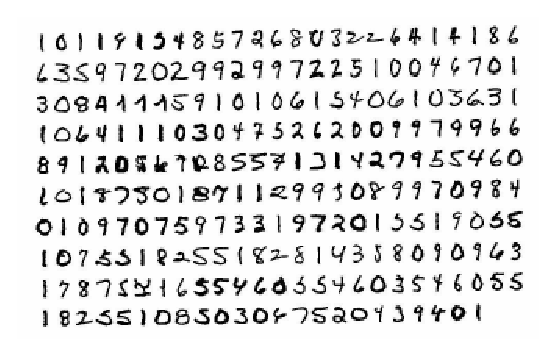
\includegraphics[width=8cm]{digit2}
      \caption{Examples of USPS digits}
      \label{digits}
    \end{minipage}

\end{figure}
\begin{figure*}[tb]
	\centering

 	\begin{tabular}{|l|l|l|l|l|l|l|l|l|l|l|}
  	\hline
  	 ~ & 0 & 1 & 2 & 3 & 4 & 5 & 6 & 7 & 8 & 9 \\ 
  	 \hline
		Training Set  & 0.16 & 0.14 & 0.1 & 0.09 & 0.09 & 0.08 & 0.09 & 0.09 & 0.07 & 0.09 \\ 
		Test Set & 0.18 & 0.13 & 0.1 & 0.08 & 0.10 & 0.08 & 0.08 & 0.07 & 0.08 & 0.09 \\
  	\hline
 		\end{tabular}
\caption{Distribution of the USPS training and test sets}
    \label{distribution}
\end{figure*}

\section{Design of Algorithms}
The $k$ nearest neighbors, as measured by each distance function, were used to predict the label for each test image. The major design steps are choosing the distance function, choosing how many nearest neighbors are considered, and choosing a method for predicting the query label based on the $k$ nearest neighbors.

\subsection{Distance functions}
\label{distancefunctions} 


Choosing a distance function is critical for $k$-nearest-neighbors. Ideally, the distance function should always return a very small value for points with the same label and very large numbers for points with different labels. The greater the separation between the intra-label and inter-label distributions, the lower the error rate of the $k$NN algorithm. 
% To assess the suitability of various distance functions for image processing, $k$NN was trained on the USPS zipcode data for each distance function and the error rates were calculated.

Five distance functions were considered: Euclidean distance, weighted Euclidean distance, similarity, weighted similarity, and Manhattan distance. The five functions are summarized in Table~\ref{tab:distfns}.

\begin{table}[b]
	\centering
	\begin{minipage}{7 cm}
		\begin{tabular}{ll}
			\toprule
			\bf{Distance Function} & $d(a,b) = \ldots$ \\
			\midrule
			Euclidean & $\left( \sum_{i=1}^m (a_i-b_i)^2 \right) ^{1/2}$ \\
			Weighted Euclidean & $ \left( w_0 + \sum_{i=1}^m w_i (a_i-b_i)^2 \right)^{1/2}$ \\
			Similarity & $1-\sum_{i=1}^m a^*_i b^*_i $ \\
			Weighted Similarity & $1-\left(w_0 + \sum_{i=1}^m w_i a^*_i b^*_i \right) $ \\
			Manhattan distance & $ \sum_{i=1}^m | a_i-b_i | $ \\
			\bottomrule
		\end{tabular}
		\caption{Overview of the $k$NN with a variety of distance functions. In each case, $a$ and $b$ represent points in $\mathbb{R}^m$, $w$ represents a weight vector in $\mathbb{R}^{m+1}$. Normalized points are expressed as in $a^* = \frac{a}{||a||_2}$. }
		\label{tab:distfns}
	\end{minipage}
\end{table}

Euclidean distance (2-norm) and Manhattan distance (1-norm) were calculated in the typical manner. Similarity was modified somewhat from the standard dot-product to fit $k$NN. First, all points were normalized to have norm 1. Next, the similarity was calculated by dot-product, yielding a similarity from -1 to 1. To allow $k$NN to operate on this function, we took $1-a\cdot b$, yielding a value in $[0,2]$, where lower values indicate closer points.

Weighted Euclidean distance and weighted similarity both required training the weights vector, $w$. This was done by minimizing an objective function via linear regression. 
For weighted similarity, the objective function was to minimize
\[ \sum_{j=1}^N \left( \hat{y}_j - w_0 - \sum_{i=1}^m w_i a_{ji} b_{ji}  \right) ^2  + \lambda \sum_{i=1}^m w_i^2 \]
over all $w$, where $\hat{y}_j$ represents the ideal similarity between points $a_j$ and $b_j$ and $N$ is the number of $(a_j,b_j)$ pairs considered during training. In this case, $\hat{y}_j$ is 1 when the labels for $x$ and $y$ match, and -1 otherwise. As explained above, the USPS training set contains 7291 images. From these, 10,000 positive examples of $(a,b)$ with matching labels were chosen at random with replacement, and 20,000 negative examples with differing labels were chosen.
%sb Is this the final number? Check.

Choosing the penalty coefficient, $\lambda$, is a difficult problem. A range of values for $\lambda$ were tested, with new weights recalculated for each. Each set of weights was used with $k$NN to predict labels for the training set (see Figure \ref{fig:lambda}).
%sb insert final number
Using this procedure we found a value of $\lambda=18$ to be optimal.
The weights associated with this $\lambda$ were then used to predict the test images. This approach is known to be susceptible to overfitting since the training data is used both for training and estimating the best value for $\lambda$. Thus, the values presented in Figure \ref{fig:lambda} are much lower than would be expected for future queries. However, assuming that the effect of overfitting is similar for all $\lambda$, this procedure is still valid for estimating the optimal $\lambda$. Furthermore, optimizing $\lambda$ is not expected to be critical for the performance of $k$NN with weighted similarity.

For weighted Euclidean distance, the objective function was to minimize
\[ \sum_{i=1}^N \left( \hat{y}_j - w_0 + \sum_{i=1}^m w_i (x_i-y_i)^2 \right)\]
over all $w$.
Here determining the ideal distance $\hat{y}$ is more difficult. It was chosen to let $\hat{y} = \sum_{i=1}^m (x_i-y_i)^2 $ for negative examples, and $\hat{y}=0$ for positive samples. This attempts to learn weights such that points with the same label will be close, while the distance between unrelated points will be unchanged. 30000 pairs of points were sampled in the same manner as for weighted similarity, and linear regression again used to determine the optimum weights for the objective function.


%sb We should only consider odd k=3,5,7...
\begin{figure}[htbp]
  \centering

    \begin{minipage}{7 cm}
      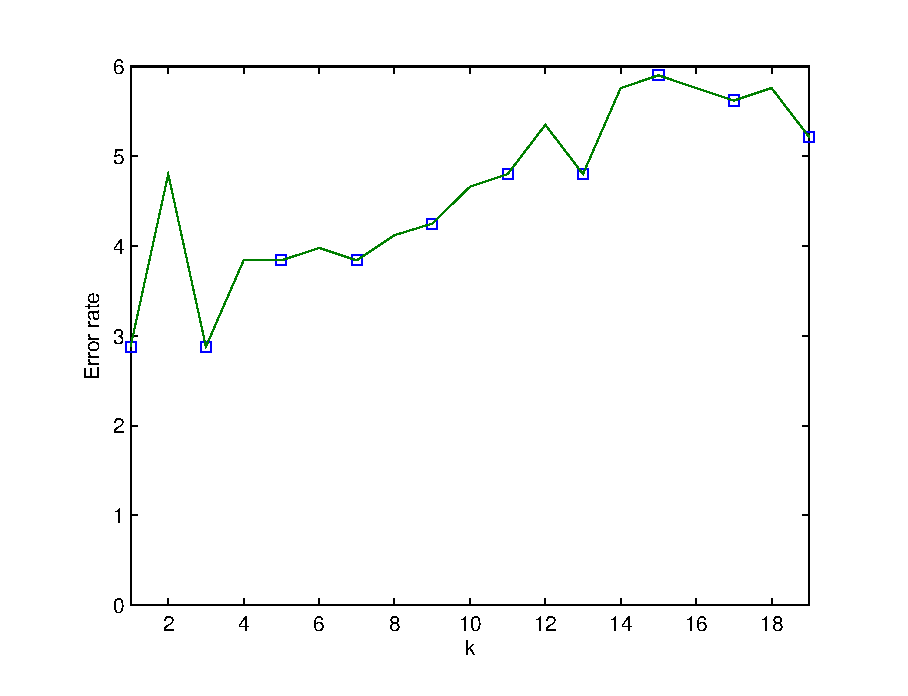
\includegraphics[width=7cm]{kerrorrate}
      %sb NOT AN ERROR RATE! Should be replotted. Also, the axis should be [0%,10%] rather than [.9, .95]
      \caption{Error rates of kNN using Euclidian distance for different $k$.}
      \label{kplots}
    \end{minipage}

\end{figure}





\subsection{Design of $k$NN classification function}
\label{kNN}
Using a desired distance function, the $k$ nearest neighbors to a test example can be found.

\subsubsection*{Choosing a label}
%Given are the $k$ closest points with their labels and the distance to the test examples.
In this project the label with plurality among the $k$ closest neighbors is selected.  If there is no single label which has a plurality, the label among the plurality-winning labels is selected that has the point with the closest distance. Further ties are broken randomly.
  
\subsubsection*{Choosing $k$}

A small odd integer is selected for $k$, because this reduces the chance of a tie when there are two labels that are overlapping in $\mathbb{R}^m$.
Selecting larger $k$ increases the probability of including non-important neighbors that are far from the target.
Choosing $k=1$ should also be avoided, since the likelihood of the closest point to the query having the wrong label is much lower than the likelihood of multiple wrong points. Thus $k=3$ was chosen as a sensible compromise.

In Figure \ref{kplots} you can see the error rates for different $k$s on the example of the Euclidean distance 

To determine the optimal value of $k$ more rigorously, $k$NN was run using Euclidean distance on 90\% of the training data. The remaining 10\% of training data was used to assess the error rate. Since the amount of training data is decreased, this procedure is expected to generate slightly poorer classifications than the full training set. The small test set also leads to increased uncertainty in accessing the true accuracy of $k$NN for each $k$. Figure \ref{kplots} shows the results. Both $k=1$ and $k=3$ give the lowest error rates.


\section{Complexity Analysis}
Selecting the nearest neighbor requires calculating the distance from each query to every training point. This takes time $\mathcal{O}(m)$ for each pair of points compared, and there are $N\cdot L$ pairs which need to be compared, where $N$ is the number of training examples and $L$ is the number of test examples. After the $k$ nearest neighbors have been identified, selecting the predicted label can be done in constant time, for a given value of $k$. Thus the overall complexity of $k$NN is $\mathcal{O}(mNL)$.

\section{Implementation}
Our implementation uses Matlab with the Lightspeed toolbox. Matrix operations were utilized wherever possible, including the optimization for Euclidean distance mentioned in \cite{elkan}. On a 2.8GHz Intel Core 2 Duo, predicting labels for the test data took 	69.79 seconds.

\section{Evaluation}
The performance of the algorithms was assessed using the error rate. The error rate of the method is defined as the percentage of labels not correctly predicted. The result are listed in Table \ref{results}. The $k$NN algorithm performed best using the Euclidean distance with 5.6\%. The similarity function and the Manhattan distance performed worse with 5.8\% respectively 6.3\%. In cases of the Euclidean distance and the similarity function weighting led to worse results probably due to overfitting. The results were significantly worse than human performance with 2.5\%. Several algorithms with better performance have been previously reported. The Covariance Support Vector Machine (\cite{shivas} performed better with 4.3\%. In 1993, Simard et al. proposed an invariant distance measure called tangent distance \cite{Simard}. The authors observed that reasonably small transformations of certain image objects does not affect class membership. Simple distance measures like the Euclidean distance do not account for this, instead they are very sensitive to affine transformations like scaling, translation, rotation or axis deformation. The tangent distance leads to better result with 2.5\%, but using 9707 instead of 7291 training examples. The best known result for 7291 training examples is based on kernel densities using the tangent distance resulting in an error rate of 2.2\% \cite{keysers}.


\begin{figure}[htbp]
	\begin{center}
		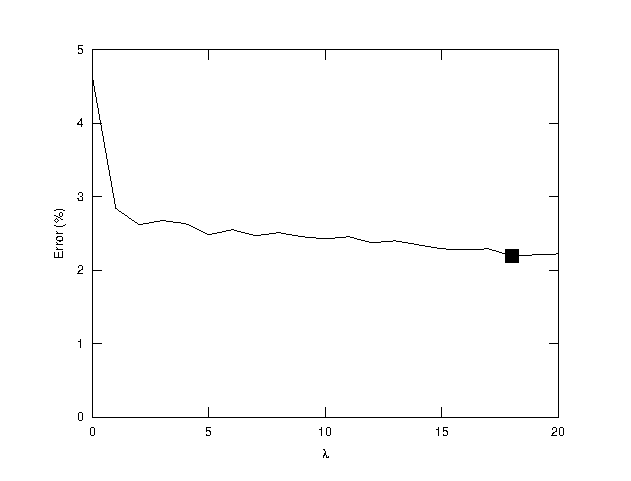
\includegraphics[scale=.8]{lambdaSelection}
		%\input{lambdaSelection.tex}
		\caption{ Error rates of $k$NN using weighted similarity with various values of $\lambda$. The optimal $\lambda=18$ is highlighted.}
		\label{fig:lambda}
	\end{center}
\end{figure}

\begin{table*}[htb]
\begin{center}
\begin{tabular}{llc}
\toprule
\bf{Method} & \bf{Distance function} & \bf{Error rate} \\
\midrule
Kernel Densities \cite{keysers} & Tangent distance & 2.2\% \\
Tangent distance \cite{Simard2}& Tangent distance& 2.5\%* \\
Human Performance \cite{Simard} & - & 2.5\%\\
Covariance Support Vector Machine \cite{shivas} & - & 4.3\%\\
$k$NN & Euclidean distance & 5.6\% \\
$k$NN & Similarity  & 5.8\% \\
$k$NN & Manhattan distance & 6.3\% \\
$k$NN & Weighted Similarity  & 6.7\% \\
$k$NN & Weighted Euclidean  & 7.7\% \\
\bottomrule
*obtained with larger dataset
\end{tabular}
\end{center}
\caption{Summary of results for the USPS dataset. Error rate of selected methods and implemented $k$NN methods with a variety of distance functions. The error rate is measured as the percentage of wrong classified test points by the algorithm. }
\label{results}
\end{table*}


%------------------------------------------------------------------------

\section{Conclusions}
Of the five distance functions implemented, Euclidean distance seems to be the best suited for clustering digit images by $k$NN. However, all distance functions were able to identify digits with high accuracy.

Choosing optimal weights for the distance functions is a difficult problem. Although the procedure used for learning weights always finds the minimum of the objective function relative to the training data, the results shown here demonstrate that the weights found are not optimum for the test examples. Weighting slightly decreases the accuracy of $k$NN for both Euclidean distance and similarity. Multiple factors may contribute to this decrease. Random fluctuations in the finite training set may lead to learning suboptimal weights. This would result in overfitting of the weighted distance functions to the training data. The errors could also be due to the necessity to sample pairs of training points while learning weights. Although 30,000 pairs were used in training, this is only 0.05\% of the possible $7291^2$ pairs. Additional coverage of the training set could increase the accuracy of weighted distance functions.

Although changing parameters and distance functions does impact the accuracy of $k$NN, all methods are able to correctly identify a very large fraction of the data. That such a simple machine learning algorithm can read digits with only 2.5\% more errors than humans is incredible.


\nocite{shivas, elkan, bishop}

{\small
\bibliographystyle{ieee}
\bibliography{egbib}
}

\end{document}
